% Dieser Text ist urheberrechtlich gesch�tzt
% Er stellt einen Auszug eines von mir erstellten Referates dar
% und darf nicht gewerblich genutzt werden
% die private bzw. Studiums bezogen Nutzung ist frei
% Nov. 2007
% Autor: Sascha Frank 
% Universit�t Freiburg 
% www.informatik.uni-freiburg.de/~frank/
\documentclass{beamer}
\setbeamertemplate{navigation symbols}{}
\usetheme{Bergen}
%\usepackage{ngerman}
%\beamersetuncovermixins{\opaqueness<1>{25}}{\opaqueness<2->{15}}

\usepackage{tikz}
\usetikzlibrary{shapes.geometric, arrows}

\usepackage[utf8]{inputenc}

\usepackage{makecell}
%\usepackage{enumitem}
\usepackage{tikz}
\tikzstyle{box2} = [draw, fill=blue!10, rounded corners, rectangle, minimum width=4cm]
\tikzstyle{box1} = [rectangle, rounded corners, minimum width=2cm, minimum height=1cm,text centered, draw=black, fill=blue!5, align=center]
\tikzstyle{arrow} = [thick, ->, >=stealth]
\usetikzlibrary{positioning}
\renewcommand\theadalign{cb}
\renewcommand\theadfont{\bfseries}
\renewcommand\theadgape{\Gape[4pt]}
\renewcommand\cellgape{\Gape[4pt]}

\usepackage{colortbl}

%\usepackage{cite}
\usepackage{caption}

\usepackage[style=numeric]{biblatex}
\addbibresource{literature.bib}

\usefonttheme[onlymath]{serif}

\usepackage{graphics}

\newcounter{saveenumi}
\newcommand{\seti}{\setcounter{saveenumi}{\value{enumi}}}
\newcommand{\conti}{\setcounter{enumi}{\value{saveenumi}}}

\resetcounteronoverlays{saveenumi}

\begin{document}
\title{Implementation of an ECC with M-511} 
\subtitle{CS448 - Introduction to IT Security}
\author{Yoann Kehler, Duong Ta}
\date{June 08, 2017} 

\begin{frame}
\titlepage
\end{frame} 

\begin{frame}{Outline}
\begin{itemize}
%	\item Recap: Elliptic Curve Cryptography with M-511
	\item How to generate a Curve?
	\item Our attempt to implement M-511
	\item Lessons Learned
\end{itemize}

\end{frame}

\begin{frame}{Structure of Elliptic Curve Cryptography}
	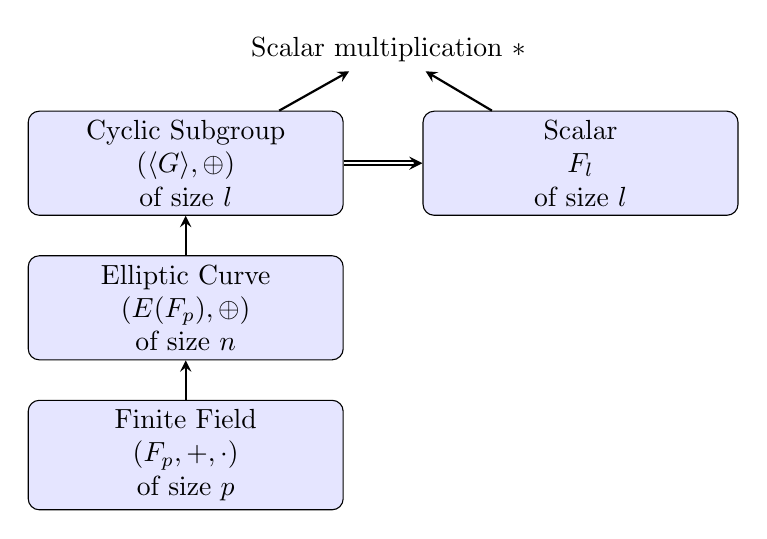
\begin{tikzpicture}
	[align=center]
	\node [box2] (f) 
	{Finite Field \\ $(\mathbb{F}_p, +, \cdot)$ \\of size $p$};
	\pause
	\node [box2](ec) 
	[above=0.5cm of f]
	{Elliptic Curve \\ $(E(\mathbb{F}_p), \oplus)$ \\of size $n$};
	\draw [arrow] (f)--(ec);
	\pause
	\node [box2](sg)
	[above=0.5cm of ec]
	{Cyclic Subgroup \\ $(\langle G\rangle, \oplus)$ \\ of size $l$};
	\draw [arrow] (ec)--(sg);
	\pause
	\node [box2](sc)
	[right=1cm of sg] 
	{Scalar \\ $\mathbb{F}_l$ \\ of size $l$};
	\draw [arrow, double] (sg)--(sc);
	\pause
	\node (sm)
	[above right=0.5cm and -1.3cm of sg]
	{Scalar multiplication $*$};
	\draw [arrow] (sg)--(sm);
	\draw [arrow] (sc)--(sm);
	\end{tikzpicture}
\end{frame} 

\begin{frame}{Structure of Elliptic Curve Cryptography}
	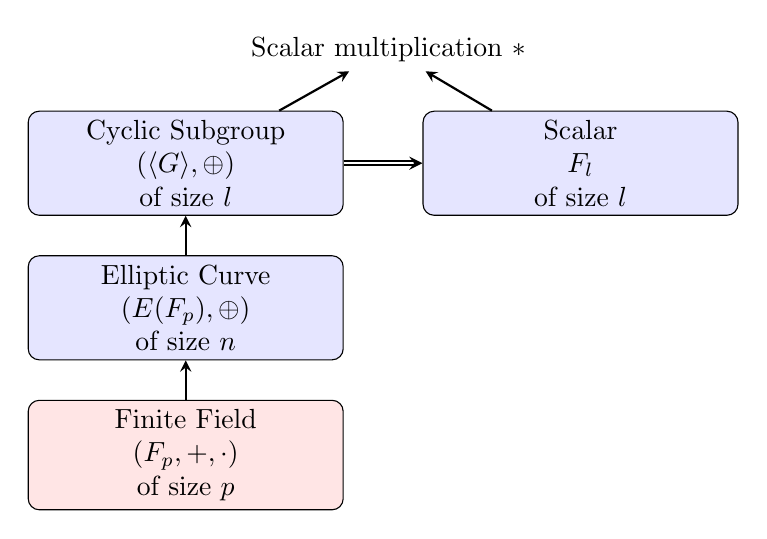
\begin{tikzpicture}
	[align=center]
	\node [box2, fill=red!10] (f) 
	{Finite Field \\ $(\mathbb{F}_p, +, \cdot)$ \\of size $p$};
	\node [box2](ec) 
	[above=0.5cm of f]
	{Elliptic Curve \\ $(E(\mathbb{F}_p), \oplus)$ \\of size $n$};
	\node [box2](sg)
	[above=0.5cm of ec]
	{Cyclic Subgroup \\ $(\langle G\rangle, \oplus)$ \\ of size $l$};
	\node [box2](sc)
	[right=1cm of sg] 
	{Scalar \\ $\mathbb{F}_l$ \\ of size $l$};
	\node (sm)
	[above right=0.5cm and -1.3cm of sg]
	{Scalar multiplication $*$};
	
	\draw [arrow] (f)--(ec);
	\draw [arrow] (ec)--(sg);
	\draw [arrow] (sg)--(sm);
	\draw [arrow] (sc)--(sm);
	\draw [arrow, double] (sg)--(sc);
	
	\end{tikzpicture}
\end{frame}

\begin{frame}{Structure of Elliptic Curve Cryptography}
	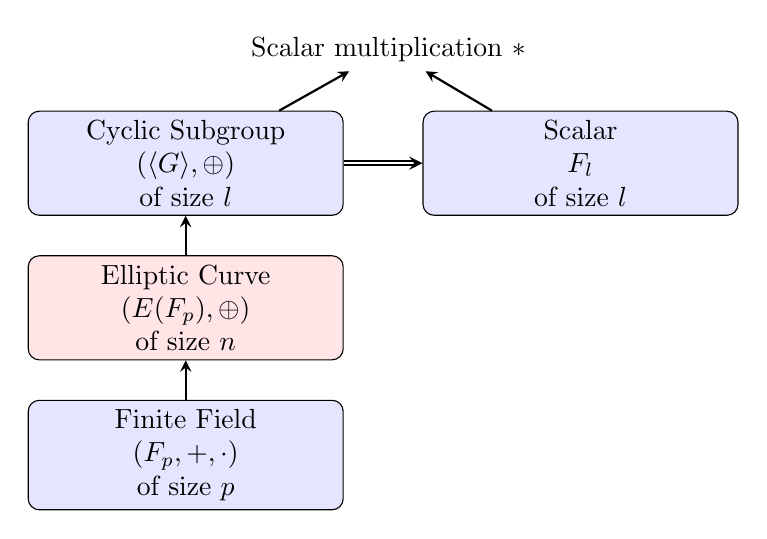
\begin{tikzpicture}
	[align=center]
	
	\node [box2] (f) 
	{Finite Field \\ $(\mathbb{F}_p, +, \cdot)$ \\of size $p$};
	\node [box2, fill=red!10](ec) 
	[above=0.5cm of f]
	{Elliptic Curve \\ $(E(\mathbb{F}_p), \oplus)$ \\of size $n$};
	\node [box2](sg)
	[above=0.5cm of ec]
	{Cyclic Subgroup \\ $(\langle G\rangle, \oplus)$ \\ of size $l$};
	\node [box2](sc)
	[right=1cm of sg] 
	{Scalar \\ $\mathbb{F}_l$ \\ of size $l$};
	\node (sm)
	[above right=0.5cm and -1.3cm of sg]
	{Scalar multiplication $*$};
	
	\draw [arrow] (f)--(ec);
	\draw [arrow] (ec)--(sg);
	\draw [arrow] (sg)--(sm);
	\draw [arrow] (sc)--(sm);
	\draw [arrow, double] (sg)--(sc);
	
	\end{tikzpicture}
\end{frame}

\begin{frame}{Generate the Elliptic Curve}
\begin{enumerate}
	\item Choose the Shapes of the curve
	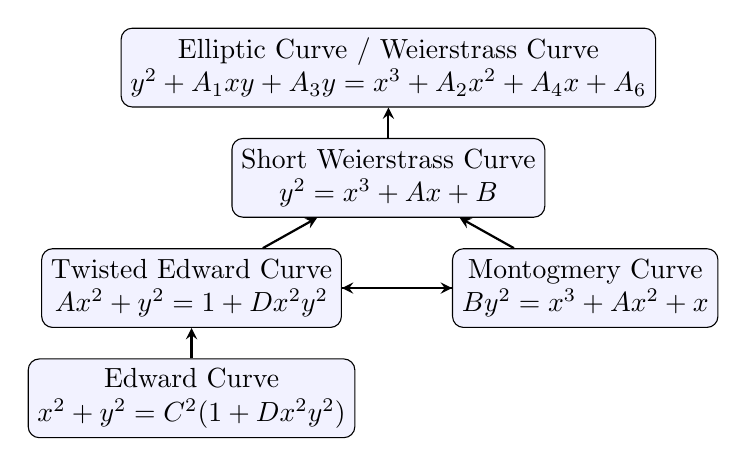
\begin{tikzpicture}[node distance= 1.4cm]
	
	\node (wc) [box1] {
		Elliptic Curve / Weierstrass Curve \\
		$y^{2}+A_{1}xy+A_{3}y=x^{3}+A_{2}x^{2}+A_{4}x+A_{6}$};
	\node (swc) [box1, below of=wc] {
		Short Weierstrass Curve\\
		$y^2=x^3+Ax+B$};
	\node (tec) [box1, below of=swc, xshift = -2.5cm] {
		Twisted Edward Curve \\
		$Ax^2+y^2=1+Dx^2y^2$};
	\node (ec) [box1, below of=tec] {
		Edward Curve\\
		$x^2+y^2=C^2(1+Dx^2y^2)$};
	\node (mc) [box1, below of=swc, xshift = 2.5cm] {
		Montogmery Curve\\
		$By^2=x^3+Ax^2+x$};
	
	\draw [arrow] (swc) -- (wc);
	\draw [arrow] (tec) -- (swc);
	\draw [arrow] (mc) -- (swc);
	\draw [arrow] (ec) -- (tec);
	\draw [arrow] (mc) -- (tec);
	\draw [arrow] (tec) -- (mc);
	\end{tikzpicture}
	Formulas from https://hyperelliptic.org/EFD \cite{hyperelliptic}
	\pause
	\item Choose parameter e.g. $A \text{ and } B \in \mathbb{F}_p$ 
	\seti
\end{enumerate}
\end{frame}
\begin{frame}{Generate the Elliptic Curve II}
\begin{enumerate}
	\conti
	\item Count number of point on the elliptic curve 
	\pause
	\[n = |E(\mathbb{F}_p)|\]
	if the curve is to small choose other parameter. 
	\item find biggest prime factor $l$ of $n$ \[n = l \cdot h\]
	\pause
	\item we call $h$ the cofactor \[h = \frac{n}{l}\]
	if the cofactor $h$ is to big/ the prime factor $l$ is to small choose other parameter.
	\seti
\end{enumerate}
\end{frame}

\begin{frame}{Structure of Elliptic Curve Cryptography}
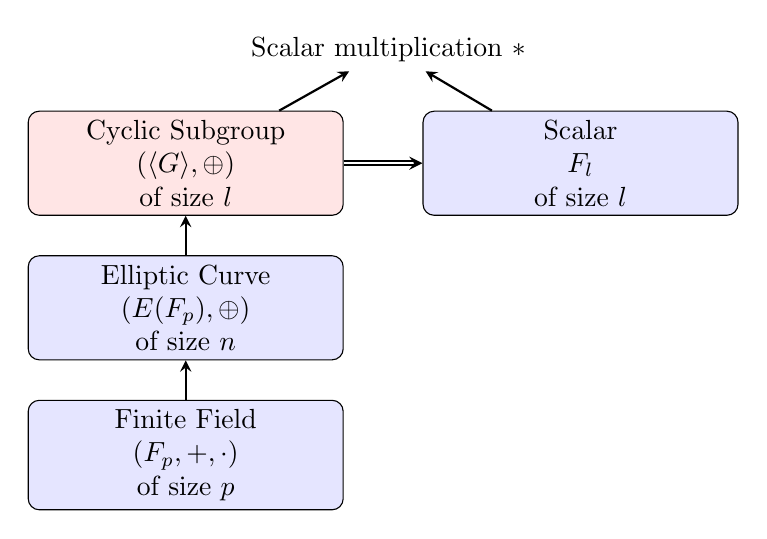
\begin{tikzpicture}
[align=center]

\node [box2] (f) 
{Finite Field \\ $(\mathbb{F}_p, +, \cdot)$ \\of size $p$};
\node [box2](ec) 
[above=0.5cm of f]
{Elliptic Curve \\ $(E(\mathbb{F}_p), \oplus)$ \\of size $n$};
\node [box2, fill=red!10](sg)
[above=0.5cm of ec]
{Cyclic Subgroup \\ $(\langle G\rangle, \oplus)$ \\ of size $l$};
\node [box2](sc)
[right=1cm of sg] 
{Scalar \\ $\mathbb{F}_l$ \\ of size $l$};
\node (sm)
[above right=0.5cm and -1.3cm of sg]
{Scalar multiplication $*$};

\draw [arrow] (f)--(ec);
\draw [arrow] (ec)--(sg);
\draw [arrow] (sg)--(sm);
\draw [arrow] (sc)--(sm);
\draw [arrow, double] (sg)--(sc);

\end{tikzpicture}
\end{frame}

\begin{frame}{Fine a big cyclic subgroup}
\begin{enumerate}
	\conti
	\item Choose random point $P$ on the curve
	\item Calculate \[G = h*P\]\\
	\[l*G = l*h*P = l \cdot \frac{n}{l} * P = n*P = O\]
	\[\Rightarrow |\langle G\rangle| = l\]
	$l$ is prime
\end{enumerate}
\end{frame}

\begin{frame}{Structure of Elliptic Curve Cryptography}
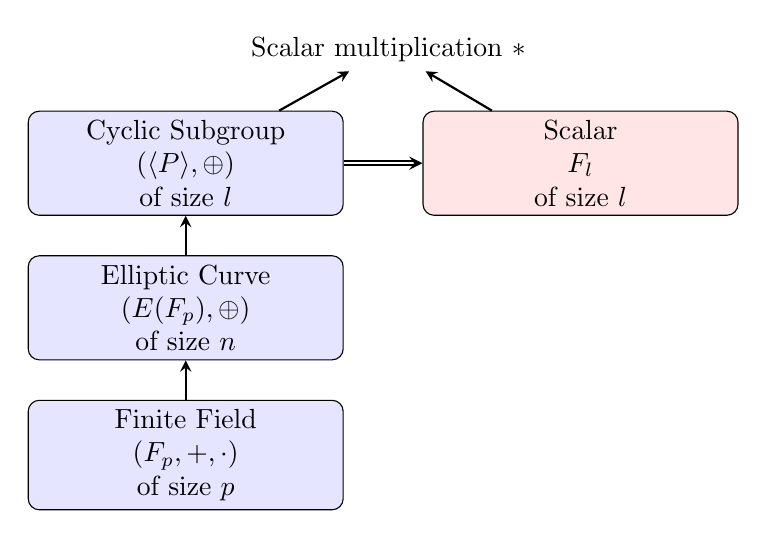
\begin{tikzpicture}
[align=center]

\node [box2] (f) 
{Finite Field \\ $(\mathbb{F}_p, +, \cdot)$ \\of size $p$};
\node [box2](ec) 
[above=0.5cm of f]
{Elliptic Curve \\ $(E(\mathbb{F}_p), \oplus)$ \\of size $n$};
\node [box2](sg)
[above=0.5cm of ec]
{Cyclic Subgroup \\ $(\langle P\rangle, \oplus)$ \\ of size $l$};
\node [box2, fill=red!10](sc)
[right=1cm of sg] 
{Scalar \\ $\mathbb{F}_l$ \\ of size $l$};
\node (sm)
[above right=0.5cm and -1.3cm of sg]
{Scalar multiplication $*$};

\draw [arrow] (f)--(ec);
\draw [arrow] (ec)--(sg);
\draw [arrow] (sg)--(sm);
\draw [arrow] (sc)--(sm);
\draw [arrow, double] (sg)--(sc);
\end{tikzpicture}
\end{frame}

\begin{frame}{The Curve M-511}
	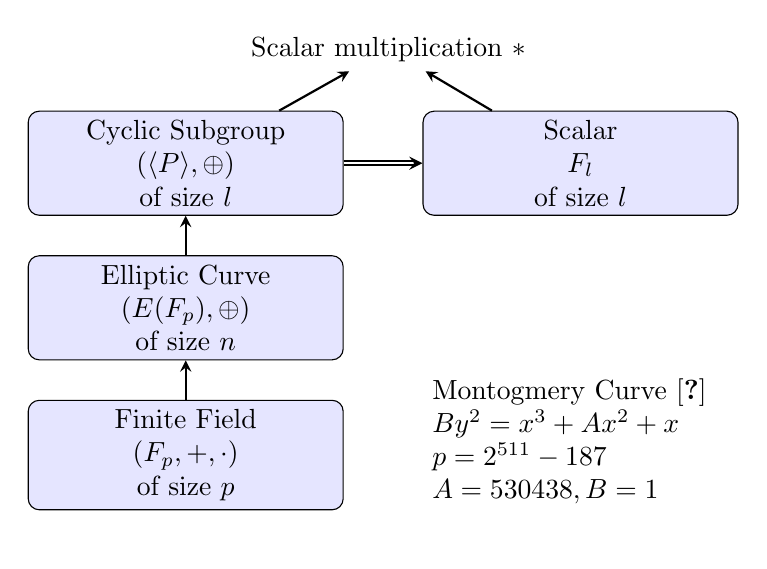
\begin{tikzpicture}
	[align=center]
	
	\node [box2] (f) 
	{Finite Field \\ $(\mathbb{F}_p, +, \cdot)$ \\of size $p$};
	\node [box2](ec) 
	[above=0.5cm of f]
	{Elliptic Curve \\ $(E(\mathbb{F}_p), \oplus)$ \\of size $n$};
	\node [box2](sg)
	[above=0.5cm of ec]
	{Cyclic Subgroup \\ $(\langle P\rangle, \oplus)$ \\ of size $l$};
	\node [box2](sc)
	[right=1cm of sg] 
	{Scalar \\ $\mathbb{F}_l$ \\ of size $l$};
	\node (sm)
	[above right=0.5cm and -1.3cm of sg]
	{Scalar multiplication $*$};
	\node (p)
	[align=left, right=1cm of f]
	{
		Montogmery Curve \cite{cryptoeprint:2013:647}\\
		$By^2=x^3+Ax^2+x$ \\
		$p = 2^{511} - 187$ \\ 
		$A = 530438, B = 1$ \\
	};
	
	\draw [arrow] (f)--(ec);
	\draw [arrow] (ec)--(sg);
	\draw [arrow] (sg)--(sm);
	\draw [arrow] (sc)--(sm);
	\draw [arrow, double] (sg)--(sc);
	\end{tikzpicture}
	$l = 2^{508} - 107247... \text{''something big''}$ \\
	$G = (5, 250041064556507... \text{''something even bigger''})$
\end{frame}

\begin{frame}{Term Project Goals}
\begin{itemize}
	\pause
	\item understand the maths behind ECC
	\pause
	\item implement a library with M-511 with:
\begin{itemize}
	\item key generation
	\item encryption and decryption
	\item signature and verification
\end{itemize}
	\pause
	\item hike Jirisan
\end{itemize}
\end{frame} 

\begin{frame}
\frametitle{Put it into practice!}
\begin{figure}[htp] \centering{
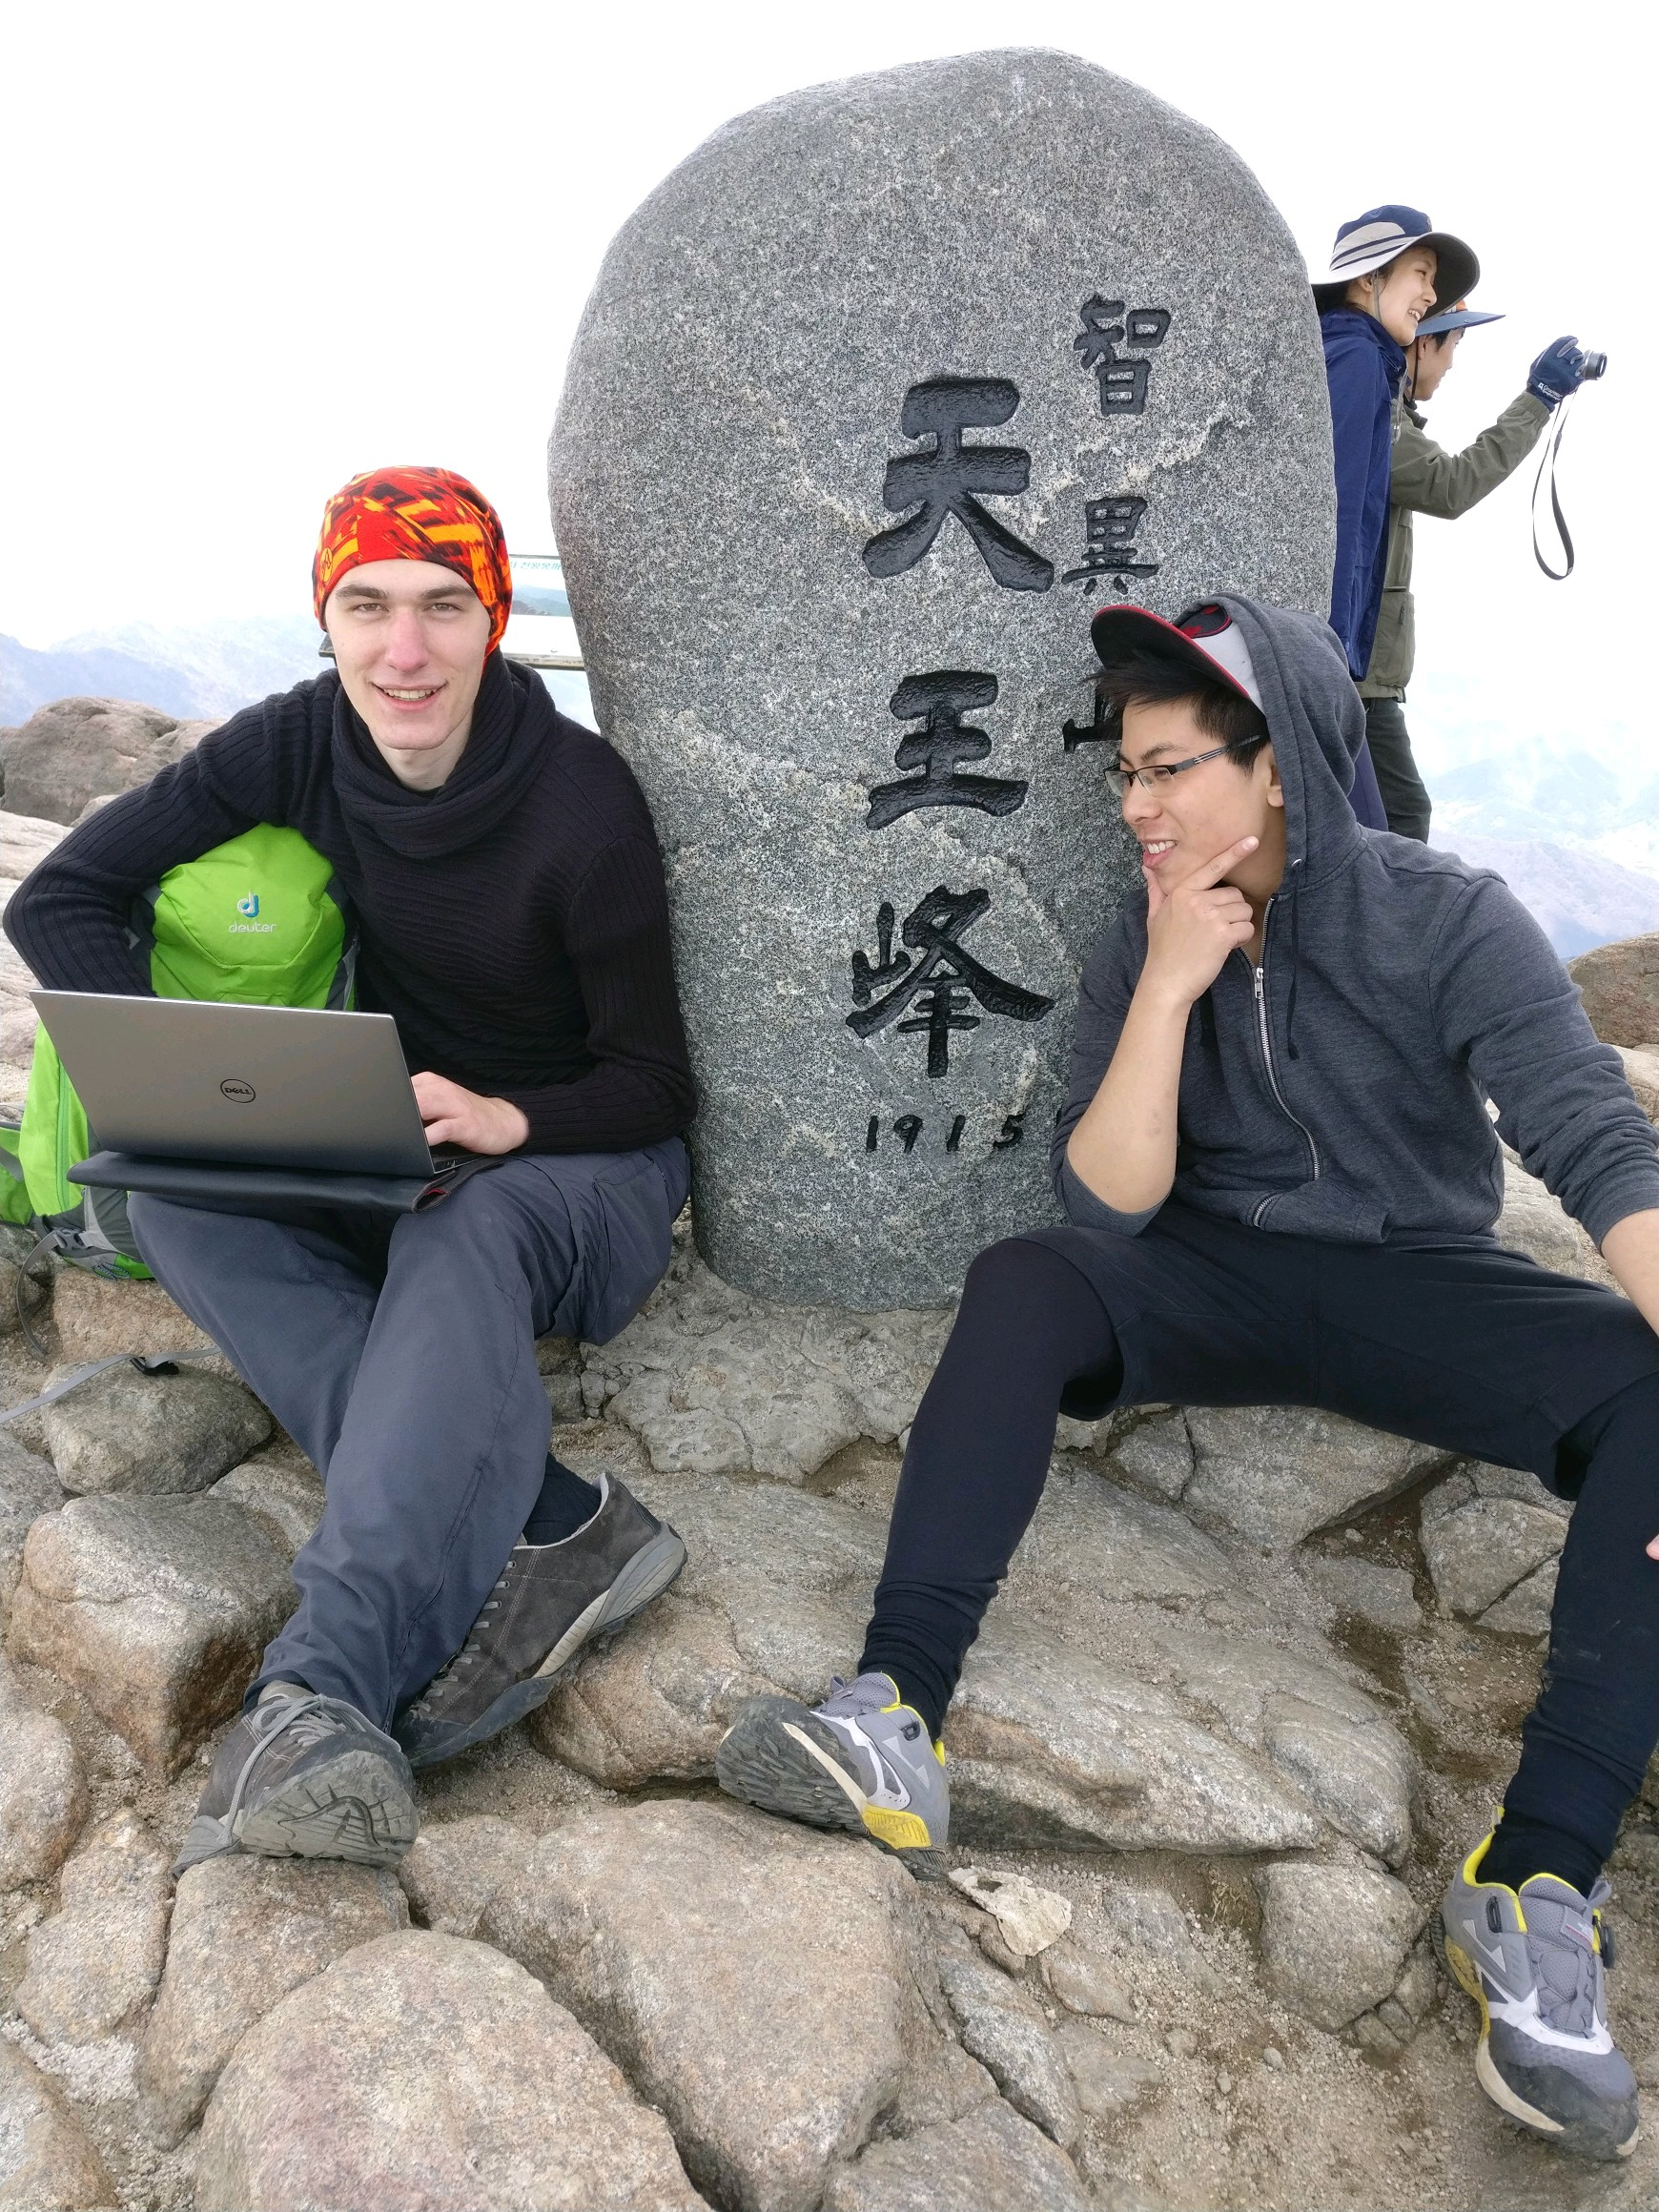
\includegraphics[scale=0.1]{img/jirisan.jpeg}}
\end{figure}  
\end{frame}


\begin{frame}
\frametitle{Architecture of our Implementation}
\begin{figure}[htp] \centering{
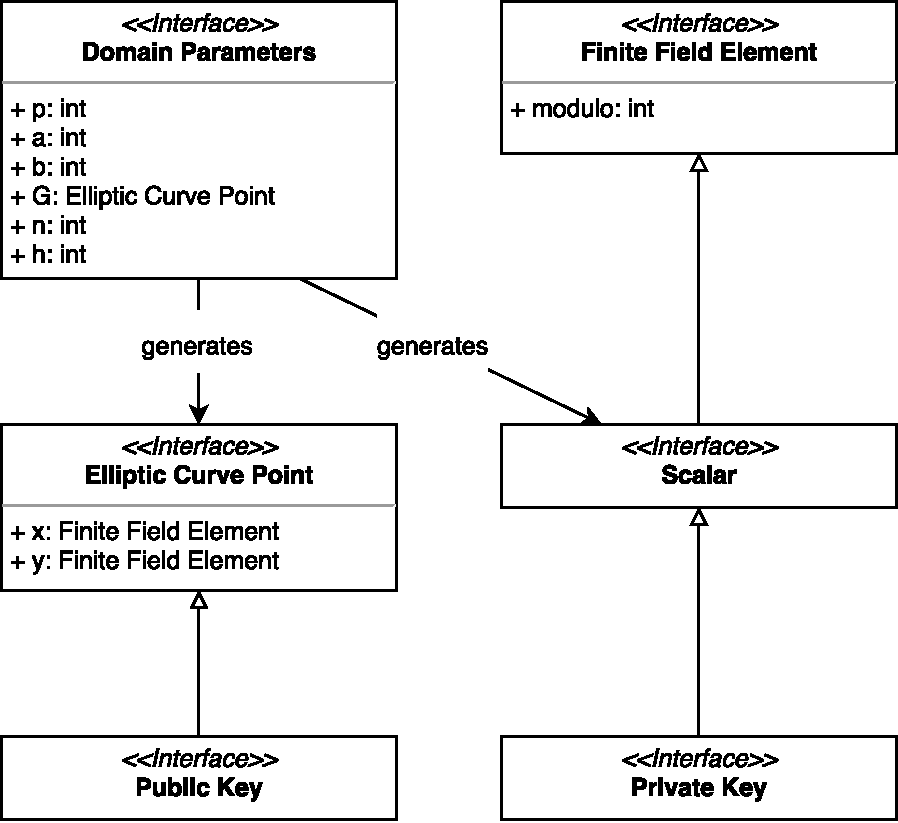
\includegraphics[scale=0.5]{img/architecture.pdf}}
\caption{Class Diagram of our Implementation}
\end{figure}  
\end{frame}

\begin{frame}{Curve Shapes}
\begin{figure}[!h]
\centering

\end{figure}
\end{frame} 

\begin{frame}[t,allowframebreaks]
	\frametitle{References}
	\printbibliography
\end{frame}

\end{document}